\documentclass[tikz,border=10pt]{standalone}
\usepackage{tikz}
\usepackage{fontawesome5}
\usepackage{amsmath,amssymb}
\usetikzlibrary{arrows.meta,positioning,fit,backgrounds,calc,shadows,shapes.geometric}

% Color definitions
\definecolor{lavenderDark}{RGB}{15, 44, 89}
\definecolor{lavenderDeep}{RGB}{10, 28, 58}
\definecolor{lavenderMedium}{RGB}{29, 78, 158}
\definecolor{lavenderLight}{RGB}{240, 246, 255}
\definecolor{lavenderBorder}{RGB}{180, 205, 237}
\definecolor{prismNavy}{RGB}{15, 44, 89}
\definecolor{prismBlue}{RGB}{29, 78, 158}
\definecolor{prismTeal}{RGB}{13, 148, 136}
\definecolor{prismGold}{RGB}{217, 119, 6}
\definecolor{prismDark}{RGB}{15, 23, 42}
\definecolor{statusFail}{RGB}{220, 38, 38}
\definecolor{cInput}{RGB}{241, 245, 249}
\definecolor{cStem}{RGB}{224, 242, 254}
\definecolor{cStage1}{RGB}{209, 250, 229}
\definecolor{cStage2}{RGB}{254, 243, 199}
\definecolor{cHead}{RGB}{219, 234, 254}

\begin{document}
% Complete Flowchart for CiviQ Legal RAG Query Processing & Translation
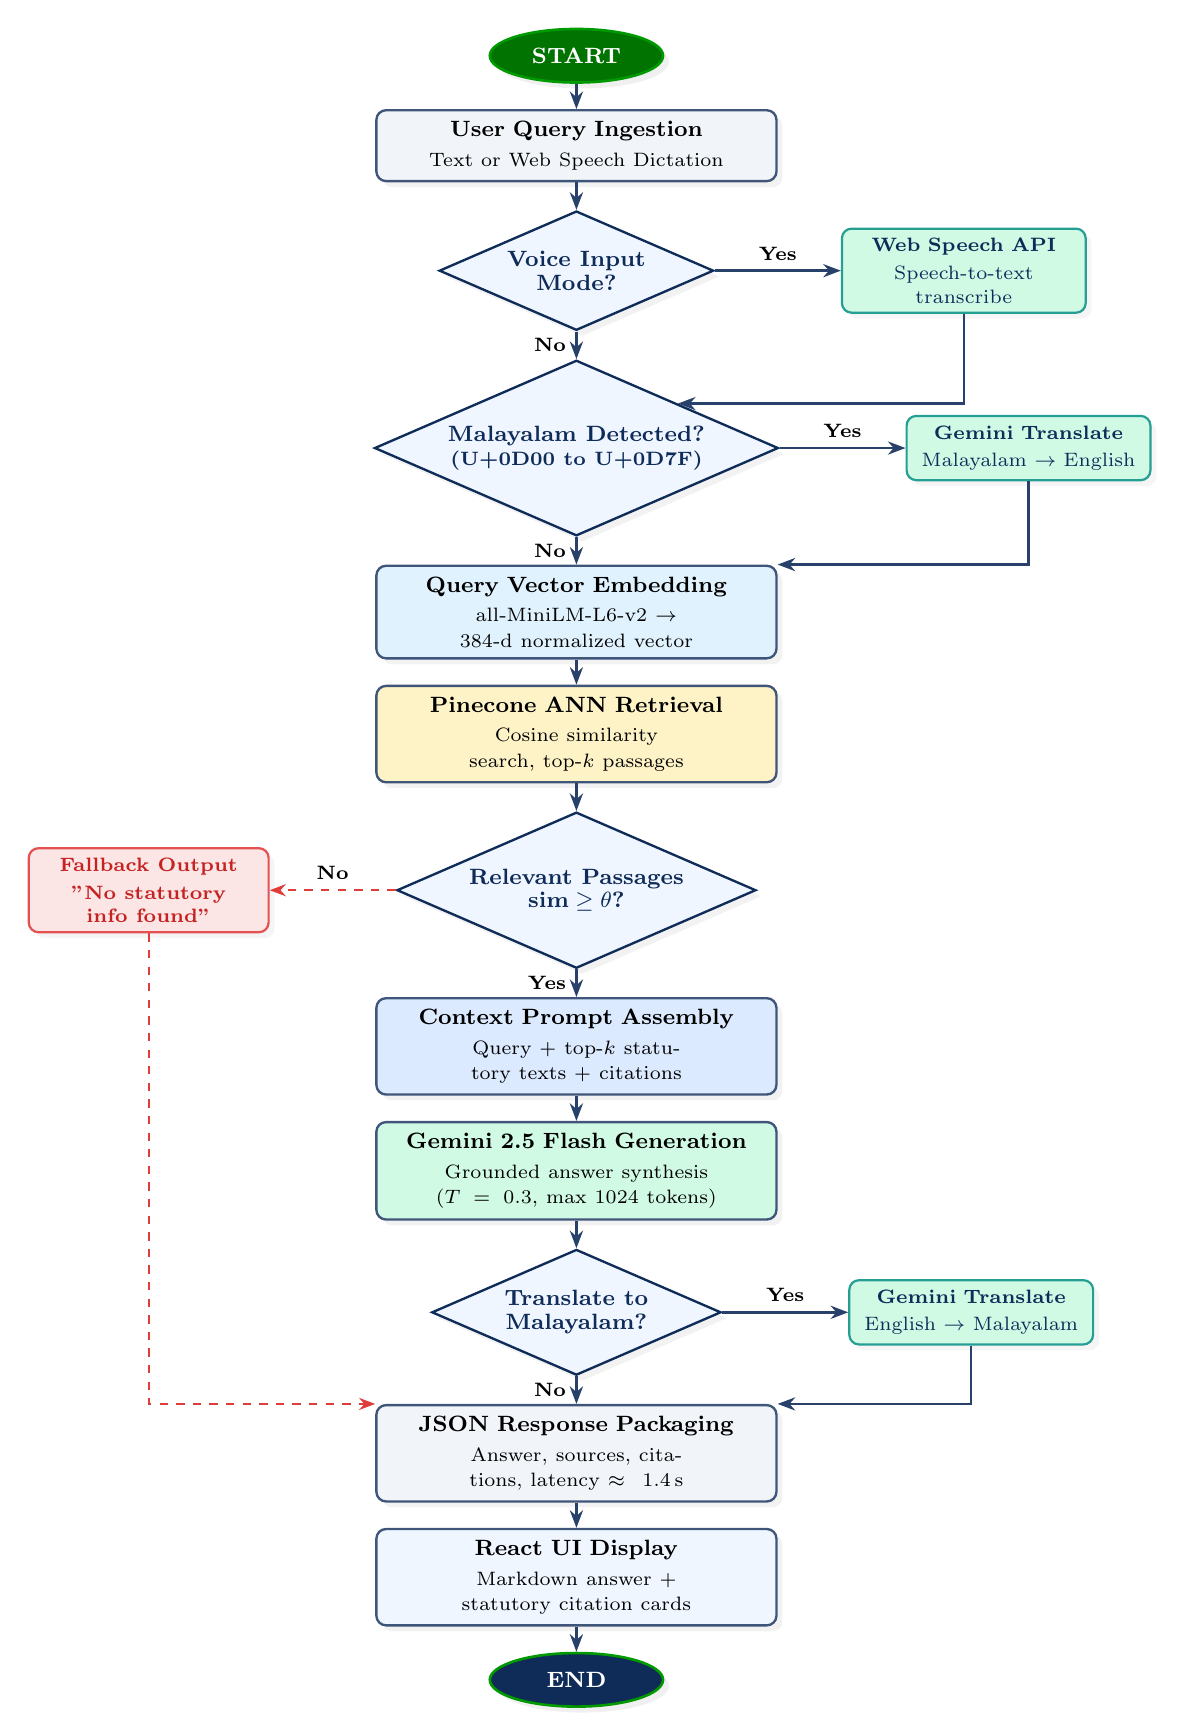
\begin{tikzpicture}[
  x=1cm, y=1cm,
  font=\sffamily,
  startend/.style={
    ellipse, draw=green!60!black, fill=green!45!black, text=white,
    line width=0.95pt, inner sep=4.0pt, font=\fontsize{8.5}{9.5}\selectfont\bfseries,
    minimum width=2.20cm, minimum height=0.68cm, drop shadow={opacity=0.12}
  },
  procbox/.style={
    rectangle, rounded corners=3.5pt,
    draw=lavenderDark!80, fill=white, text=black,
    line width=0.85pt, inner sep=4.0pt, font=\fontsize{8.0}{9.2}\selectfont,
    minimum height=0.72cm, text width=4.80cm, align=center, drop shadow={opacity=0.10}
  },
  decision/.style={
    diamond, aspect=2.3,
    draw=prismNavy, fill=lavenderLight, text=prismNavy,
    line width=0.85pt, inner sep=2.5pt, font=\fontsize{7.6}{8.6}\selectfont\bfseries,
    align=center, drop shadow={opacity=0.10}
  },
  sidebox/.style={
    rectangle, rounded corners=3.5pt,
    draw=prismTeal!90, fill=cStage1, text=prismNavy,
    line width=0.80pt, inner sep=3.5pt, font=\fontsize{7.5}{8.5}\selectfont,
    minimum height=0.66cm, text width=2.85cm, align=center, drop shadow={opacity=0.08}
  },
  errorbox/.style={
    rectangle, rounded corners=3.5pt,
    draw=statusFail!80, fill=statusFail!12, text=statusFail!90!black,
    line width=0.80pt, inner sep=3.5pt, font=\fontsize{7.5}{8.5}\selectfont\bfseries,
    minimum height=0.66cm, text width=2.80cm, align=center, drop shadow={opacity=0.08}
  },
  flowarr/.style={
    -{Stealth[scale=0.90]}, line width=0.90pt, draw=lavenderDark!90
  },
  failarr/.style={
    -{Stealth[scale=0.85]}, line width=0.85pt, draw=statusFail!90, dashed
  }
]

  % Central Column - Main Processing Flow
  \node[startend] (start) at (0, 11.20) {START};

  \node[procbox, fill=cInput, below=0.32cm of start] (user_in) {%
    \textbf{User Query Ingestion}\\[1.5pt]
    {\fontsize{7.0}{8.0}\selectfont Text or Web Speech Dictation}%
  };

  \node[decision, below=0.35cm of user_in] (d_voice) {%
    Voice Input\\Mode?%
  };

  \node[decision, below=0.35cm of d_voice] (d_lang) {%
    Malayalam Detected?\\{\fontsize{6.8}{7.8}\selectfont (U+0D00 to U+0D7F)}%
  };

  \node[procbox, fill=cStem, below=0.35cm of d_lang] (embed) {%
    \textbf{Query Vector Embedding}\\[1.5pt]
    {\fontsize{7.0}{8.0}\selectfont all-MiniLM-L6-v2 $\to$ 384-d normalized vector}%
  };

  \node[procbox, fill=cStage2, below=0.32cm of embed] (pinecone) {%
    \textbf{Pinecone ANN Retrieval}\\[1.5pt]
    {\fontsize{7.0}{8.0}\selectfont Cosine similarity search, top-$k$ passages}%
  };

  \node[decision, below=0.35cm of pinecone] (d_match) {%
    Relevant Passages\\$\text{sim} \ge \theta$?%
  };

  \node[procbox, fill=cHead, below=0.35cm of d_match] (prompt_bld) {%
    \textbf{Context Prompt Assembly}\\[1.5pt]
    {\fontsize{7.0}{8.0}\selectfont Query + top-$k$ statutory texts + citations}%
  };

  \node[procbox, fill=cStage1, below=0.32cm of prompt_bld] (gemini) {%
    \textbf{Gemini 2.5 Flash Generation}\\[1.5pt]
    {\fontsize{7.0}{8.0}\selectfont Grounded answer synthesis ($T=0.3$, max 1024 tokens)}%
  };

  \node[decision, below=0.35cm of gemini] (d_trans_back) {%
    Translate to\\Malayalam?%
  };

  \node[procbox, fill=cInput, below=0.35cm of d_trans_back] (respond) {%
    \textbf{JSON Response Packaging}\\[1.5pt]
    {\fontsize{7.0}{8.0}\selectfont Answer, sources, citations, latency $\approx 1.4$\,s}%
  };

  \node[procbox, fill=lavenderLight, below=0.32cm of respond] (render) {%
    \textbf{React UI Display}\\[1.5pt]
    {\fontsize{7.0}{8.0}\selectfont Markdown answer + statutory citation cards}%
  };

  \node[startend, fill=lavenderDark, below=0.32cm of render] (end) {END};

  % Side Branches (Left/Right)
  % 1. Voice transcription (Right of d_voice)
  \node[sidebox, right=1.60cm of d_voice] (voice_stt) {%
    \textbf{Web Speech API}\\[1.5pt]
    {\fontsize{7.0}{8.0}\selectfont Speech-to-text transcribe}%
  };

  % 2. Translation to English (Right of d_lang)
  \node[sidebox, right=1.60cm of d_lang] (trans_en) {%
    \textbf{Gemini Translate}\\[1.5pt]
    {\fontsize{7.0}{8.0}\selectfont Malayalam $\to$ English}%
  };

  % 3. No match error (Left of d_match)
  \node[errorbox, left=1.60cm of d_match] (no_match) {%
    \textbf{Fallback Output}\\[1.5pt]
    {\fontsize{7.0}{8.0}\selectfont "No statutory info found"}%
  };

  % 4. Translation to Malayalam (Right of d_trans_back)
  \node[sidebox, right=1.60cm of d_trans_back] (trans_ml) {%
    \textbf{Gemini Translate}\\[1.5pt]
    {\fontsize{7.0}{8.0}\selectfont English $\to$ Malayalam}%
  };

  % Downward Connections
  \draw[flowarr] (start) -- (user_in);
  \draw[flowarr] (user_in) -- (d_voice);
  \draw[flowarr] (d_voice) -- node[left, font=\fontsize{7.2}{8.2}\selectfont\bfseries]{No} (d_lang);
  \draw[flowarr] (d_lang) -- node[left, font=\fontsize{7.2}{8.2}\selectfont\bfseries]{No} (embed);
  \draw[flowarr] (embed) -- (pinecone);
  \draw[flowarr] (pinecone) -- (d_match);
  \draw[flowarr] (d_match) -- node[left, font=\fontsize{7.2}{8.2}\selectfont\bfseries]{Yes} (prompt_bld);
  \draw[flowarr] (prompt_bld) -- (gemini);
  \draw[flowarr] (gemini) -- (d_trans_back);
  \draw[flowarr] (d_trans_back) -- node[left, font=\fontsize{7.2}{8.2}\selectfont\bfseries]{No} (respond);
  \draw[flowarr] (respond) -- (render);
  \draw[flowarr] (render) -- (end);

  % Branch: Voice transcription
  \draw[flowarr] (d_voice.east) -- node[above, font=\fontsize{7.2}{8.2}\selectfont\bfseries]{Yes} (voice_stt.west);
  \draw[flowarr] (voice_stt.south) |- (d_lang.north east);

  % Branch: Translation to English
  \draw[flowarr] (d_lang.east) -- node[above, font=\fontsize{7.2}{8.2}\selectfont\bfseries]{Yes} (trans_en.west);
  \draw[flowarr] (trans_en.south) |- (embed.north east);

  % Branch: Fallback when no match
  \draw[failarr] (d_match.west) -- node[above, font=\fontsize{7.2}{8.2}\selectfont\bfseries]{No} (no_match.east);
  \draw[failarr] (no_match.south) |- (respond.north west);

  % Branch: Translation to Malayalam
  \draw[flowarr] (d_trans_back.east) -- node[above, font=\fontsize{7.2}{8.2}\selectfont\bfseries]{Yes} (trans_ml.west);
  \draw[flowarr] (trans_ml.south) |- (respond.north east);

\end{tikzpicture}
\end{document}
